%preamble
\documentclass[letterpaper]{article}
\synctex=1

\usepackage{listings}
\lstset{
%language=Assembler
% breaklines=true
%frame=single,
%xleftmargin=-1pt
}
\usepackage{geometry}
\usepackage{array}
\usepackage{lipsum}

\usepackage{graphicx}
\usepackage{float}
\graphicspath{ {images/} }
%
% \newenvironment{changemargin}[2]{%
% \begin{list}{}{%
% \setlength{\topsep}{0pt}%
% \setlength{\leftmargin}{#1}%
% \setlength{\rightmargin}{#2}%
% \setlength{\listparindent}{\parindent}%
% \setlength{\itemindent}{\parindent}%
% \setlength{\parsep}{\parskip}%
% }%
% \item[]}{\end{list}}

% \usepackage{tabu}
%actual document
\begin{document}

  %titlepage
  \begin{titlepage}
    \begin{center}

      \LARGE
      ECE 212 Lab - Introduction to Microprocessors

      Department of Electrical and Computer Engineering

      University of Alberta

      \vspace{2cm}

      Lab 1: Introduction to Assembly Language.

      \vspace{5cm}
      \Large

      \begin{tabular}{ | m{5cm} | m{5cm} | }
        \hline
        Student Name & Student \\
        \hline
        Arun Woosaree & xxxxxxx \\
        \hline
        Navras Kamal & 1505463 \\
        \hline
      \end{tabular}


      % \begin{tabu} to 0.8\textwidth{  | X[c] | X[c] | }
      %   \hline
      %   Student Name & Student \\
      %   \hline
      %   Arun Woosaree & xxxxxxx \\
      %   \hline
      %   Navras Kamal & 1505463 \\
      %   \hline
      % \end{tabu}


    \end{center}
\end{titlepage}

%table of tableofcontents

\tableofcontents

% \vfill
\newpage

\section{Introduction}
  This text is filler text from an ece 210 lab report
  The purpose of this experiment was to explore the process behind designing and implementing real life design problems using the Xilinx software. A multiplexer (MUX) and demultiplexer (DEMUX) circuit were designed with the goal of sending data to three different 'radio astronomers'. Xilinx was used to create schematics for the circuit, which was then programmed to the Xilinx FPGA development board. The second part of the experiment involved the design and implementation of a lab access control circuit, again using Xilinx and the development board.

  A multiplexer is a device that selects a single input from multiple signals, and only transmits one signal. It effectively receives multiple inputs, and only has a single output. The selection occurs based on the values of the 'selection signals'. For a 2x1 (two input signals) multiplexer, only one select signal is needed, but for a 4x1 multiplexer, two select signals are needed.

  Multiplexers are often coupled with demultiplexers. DEMUXs receive a single input, and then send this input on to different possible outputs or 'locations', based again on the select signals inputted. The combination of a multiplexer and a demultiplexer allow the transfer of multiple signals over a shared medium or transmission line, in a process known as multiplexing. The signals are combined at the transmitter by the MUX and then split up at the receiving end by the DEMUX.

  In the lab, the Xilinx software was utilized to design a three input/one output MUX, and a one input/three output DEMUX using only AND gates, OR gates, and inverters. Initially, Boolean expressions representing the MUX and DEMUX were simplified using a K-Map. From these simplified expressions, two separate designs were created using schematic capture tools, and then were utilized to implement data transmission to engineers. The output of the MUX was wired to the input of the DEMUX. The three outputs from the DEMUX are then sent to the office of radio astronomers. Three additional outputs are used, (designated as 'engineering indicators') to confirm the radio astronomers are receiving data. Only one of these engineering indicators should be turned on, considering the DEMUX selects only one output.

  In the second part of the experiment, a circuit was designed and then implemented to
  control access to two labs: Lab0 and Lab1. Two input signals are accepted
  (a 2-bit card code and a 3-bit key), with three output signals (Lab0\textunderscore unlock, Lab1\textunderscore unlock, and Alarm).
   A valid card read and correct key entered unlocks the appropriate lab, and
   invalid input signals will sound the alarm.


\section{Design}
  \subsection{Part A}
    For the first part of the lab, the address register a1 was chosen to initially point to
    memory location 0x2300000, which is the starting point of where the input data was stored.
    We used this address register to keep track of the memory location of the next long word
    of data to be read as an input to our program. Even though one memory location is capable
    of storing one ASCII character, in this lab, 4 memory locations were used to store one
    ASCII character, as specified in the lab manual.
    Next, a2 was selected to initially point at the memory location 0x231000, which is the
    starting location of where our output for the converted values was. This register
    was used to keep track of the memory location of where the next long word of
    our converted data would go. The data register d2 was chosen to temporarily store
    data so we could do comparisons and process the input data.
    The \textit{Setzeros.s} and the \textit{DataSrorage.s}
    files, which were provided, were used to initialize memory contents.

    We started with a loop branch that served as our main looping function. This
    loop first starts by moving data from a memory location pointed to by a1, to
    the data register d2 so that we could start comparing the input data to known ASCII values.
    In the first comparison, the input character is compared to `0x0D', which is the ASCII
    code for the `Enter' key. This code is meant to signal the end of the program, so if
    the input was the ASCII code for `Enter', we branched to a label that
    would end our program. The next step was to determine if the input character was valid.
    For Part A, an input character was valid if it was an ASCII character from 0-9, A-F, or a-f.
    In other words, the data was accepted if it was in the following ranges: 0x30-0x39,
    0x41-0x46, or 0x61-0x66. If the input character was invalid, we brached to a label
    named `err', which would put the error code `FFFFFFFF' in the memory location
    pointed to by a2, which keeps track of where our output data goes.

    If the input character was valid, we had three branches to take care of each
    of the accepted ranges of input. For example, in the branch that took care of the
    input range A-F, the ASCII value of `A' was subtracted from the input value, and
    the difference was added to the hex value 0xA. The converted value is then moved
    to the memory location pointed to by a2, which keeps track of where our output data goes.
    Similar steps were done to convert input characters in the other accepted ranges.
    After converting the input character and moving the output to the location pointed by a2,
    we branched to a label `endloop', which increments the addresses stored in a1 and a2 by 4,
    and then branches to the loop, where the process is repeated. The flowchart diagram can
    be found in the Appendix.

    % \begin{figure}
    %   \includegraphics{/path/to/figure}
    %   \caption{}
    %   \label{}
    % \end{figure}

    \subsubsection{Part A Sample Calculation of Conversion}
      TODO

  \subsection{Part B}
    The design for Part B was very similar to Part A. The address register a1 still
    initially points to 0x2300000, but this time, a2 now points to 0x2320000, which is
    where the converted data is stored.The same data register d2 was used to temporarily
    store the input and process the data. Just like in Part A, the \textit{Setzeros.s} and the \textit{DataSrorage.s} files
    were used to initialize memory contents as well.

    Once again, we had a loop branch that initially loads input data from the location
    pointed to by a1 into data register d2, and the ASCII `Enter' code still terminates
    the program, as before. In Part B, valid inputs are the ASCII characters A-Z and a-z.
    (0x41-0x5A and 0x61-0x7A)
    Error handling was also similar to Part A, where the value 0xFFFFFFFF was stored at the
    memory location pointed to by a2. We had two branches to handle the two ranges of accepted
    characters.

    For example, if an input character was in the range a-z, a difference was taken
    relative to the ASCII character `a', and added to the ASCII character `A'. The
    converted value is then stored at the memory location pointed to by a2, and
    the addresses stored in a1 and a2 are incremented by 4 before the loop
    starts over. The flowchart diagram can be found in the Appendix.

    % \begin{figure}
    %   \includegraphics{/path/to/figure}
    %   \caption{}
    %   \label{}
    % \end{figure}

    \subsubsection{Part B Sample Calculation of Conversion}
      TODO

\section{Testing}
  \subsection{Part A}
    Initially, we visually tested our code by using the debugger in Eclipse IDE.
    While stepping through the code, we would check the values at relevant memory
    locations, and the data and address registers. When the bugs were ironed out,
    we went on to the next phase of testing.
    Our code was tested using the provided \textit{Lab1Test.s} file. More specifically,
    this program was moved into the project folder, downloaded to the ColdFire microcontroller,
    and the MTTTY serial monitor was loaded to monitor the expected output. Our code was
    further tested by replacing the `DataStorage.s' file with the other variants provided
    named: \textit{DataStorage1.s}, \textit{DataStorage2.s}, and \textit{DataStorage3.s}.
    Finally, our program, which produced the correct output, was verified by a lab TA.

    \begin{figure}[h!]
      \centering
      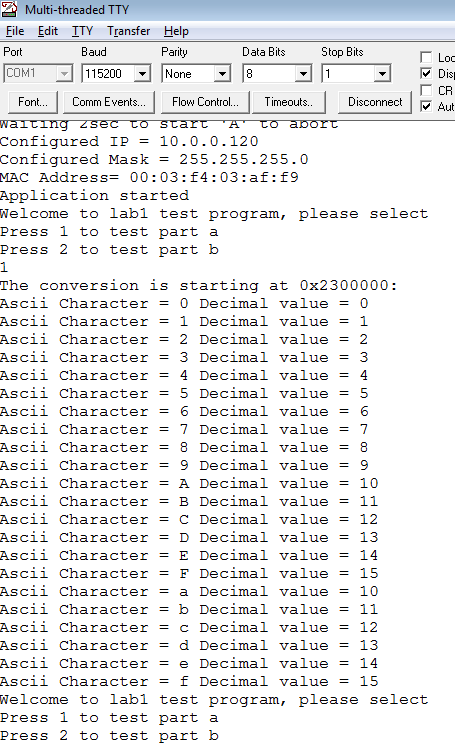
\includegraphics[width=0.4\textwidth]{tst1a.png}
      \caption{MTTTY output when testing our Part A solution}
    \end{figure}

  \subsection{Part B}
    The procedure for testing our code for part B was very similar to the process
    described above in Part A. We visually inspected our code in the Eclipse IDE,
    used the Eclipse debugger to step through our code, and monitor relevant
    memory addresses and registers. When we were confident that we had a working
    solution, we used the provided files \textit{Lab1Test.s}, and the \textit{DataStorage*.s}
    files to verify our solution by downloading the program to the ColdFire microcontroller,
    and monitoring the output in MTTTY. Finally, our solution was verified by a lab TA.

    \begin{figure}[h!]
      \centering
      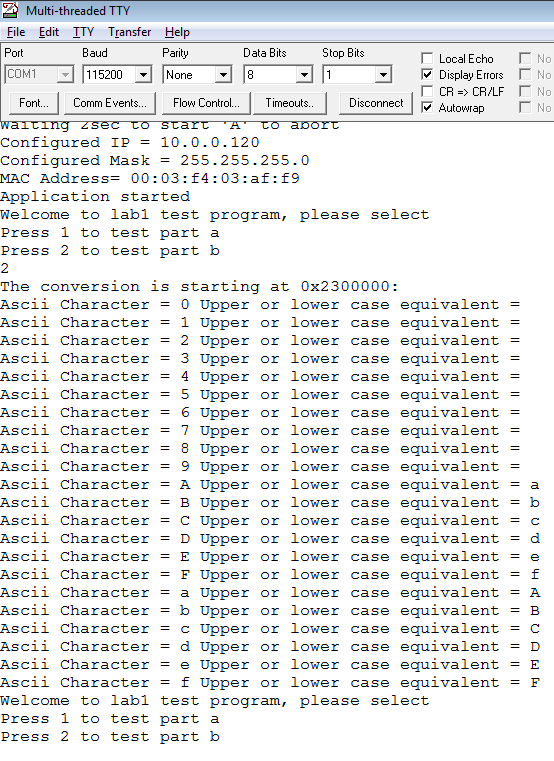
\includegraphics[width=0.4\textwidth]{tst1b.png}
      \caption{MTTTY output when testing our Part B solution}
    \end{figure}

\section{Questions}

    \subsection{Question 1}
      \textit{``What happens when there is no exit code ‘0x0D’ provided in the initialization process? Would it cause a problem? Why or why not?''}
      \\ \\
      \noindent\textbf{A:}
      % \lipsum[7]
      It would cause an infinite loop, yo

    \subsection{Question 2}
      \textit{``How can our code be modified to provide a variable address range? For example, what if I only wanted to convert the first 10 data entires? ''}
      \\ \\
      \noindent\textbf{A:}
      % \lipsum[8]
      You could, like, use a counter in d2, or maybe a stack idk

\section{Conclusion}
  \lipsum[9]
  \medskip
  \lipsum[10]

\newpage
\section{Appendix}
  %\textwidth=600pt
  \subsection{Part A Assembler Code}
    % \begin{changemargin}{-2cm}{-2cm}
    \lstinputlisting{parta.s}
  % \end{changemargin}
\newpage
  \subsection{Part A Flowchart Diagram}
    \begin{figure}[h!]
      \centering
      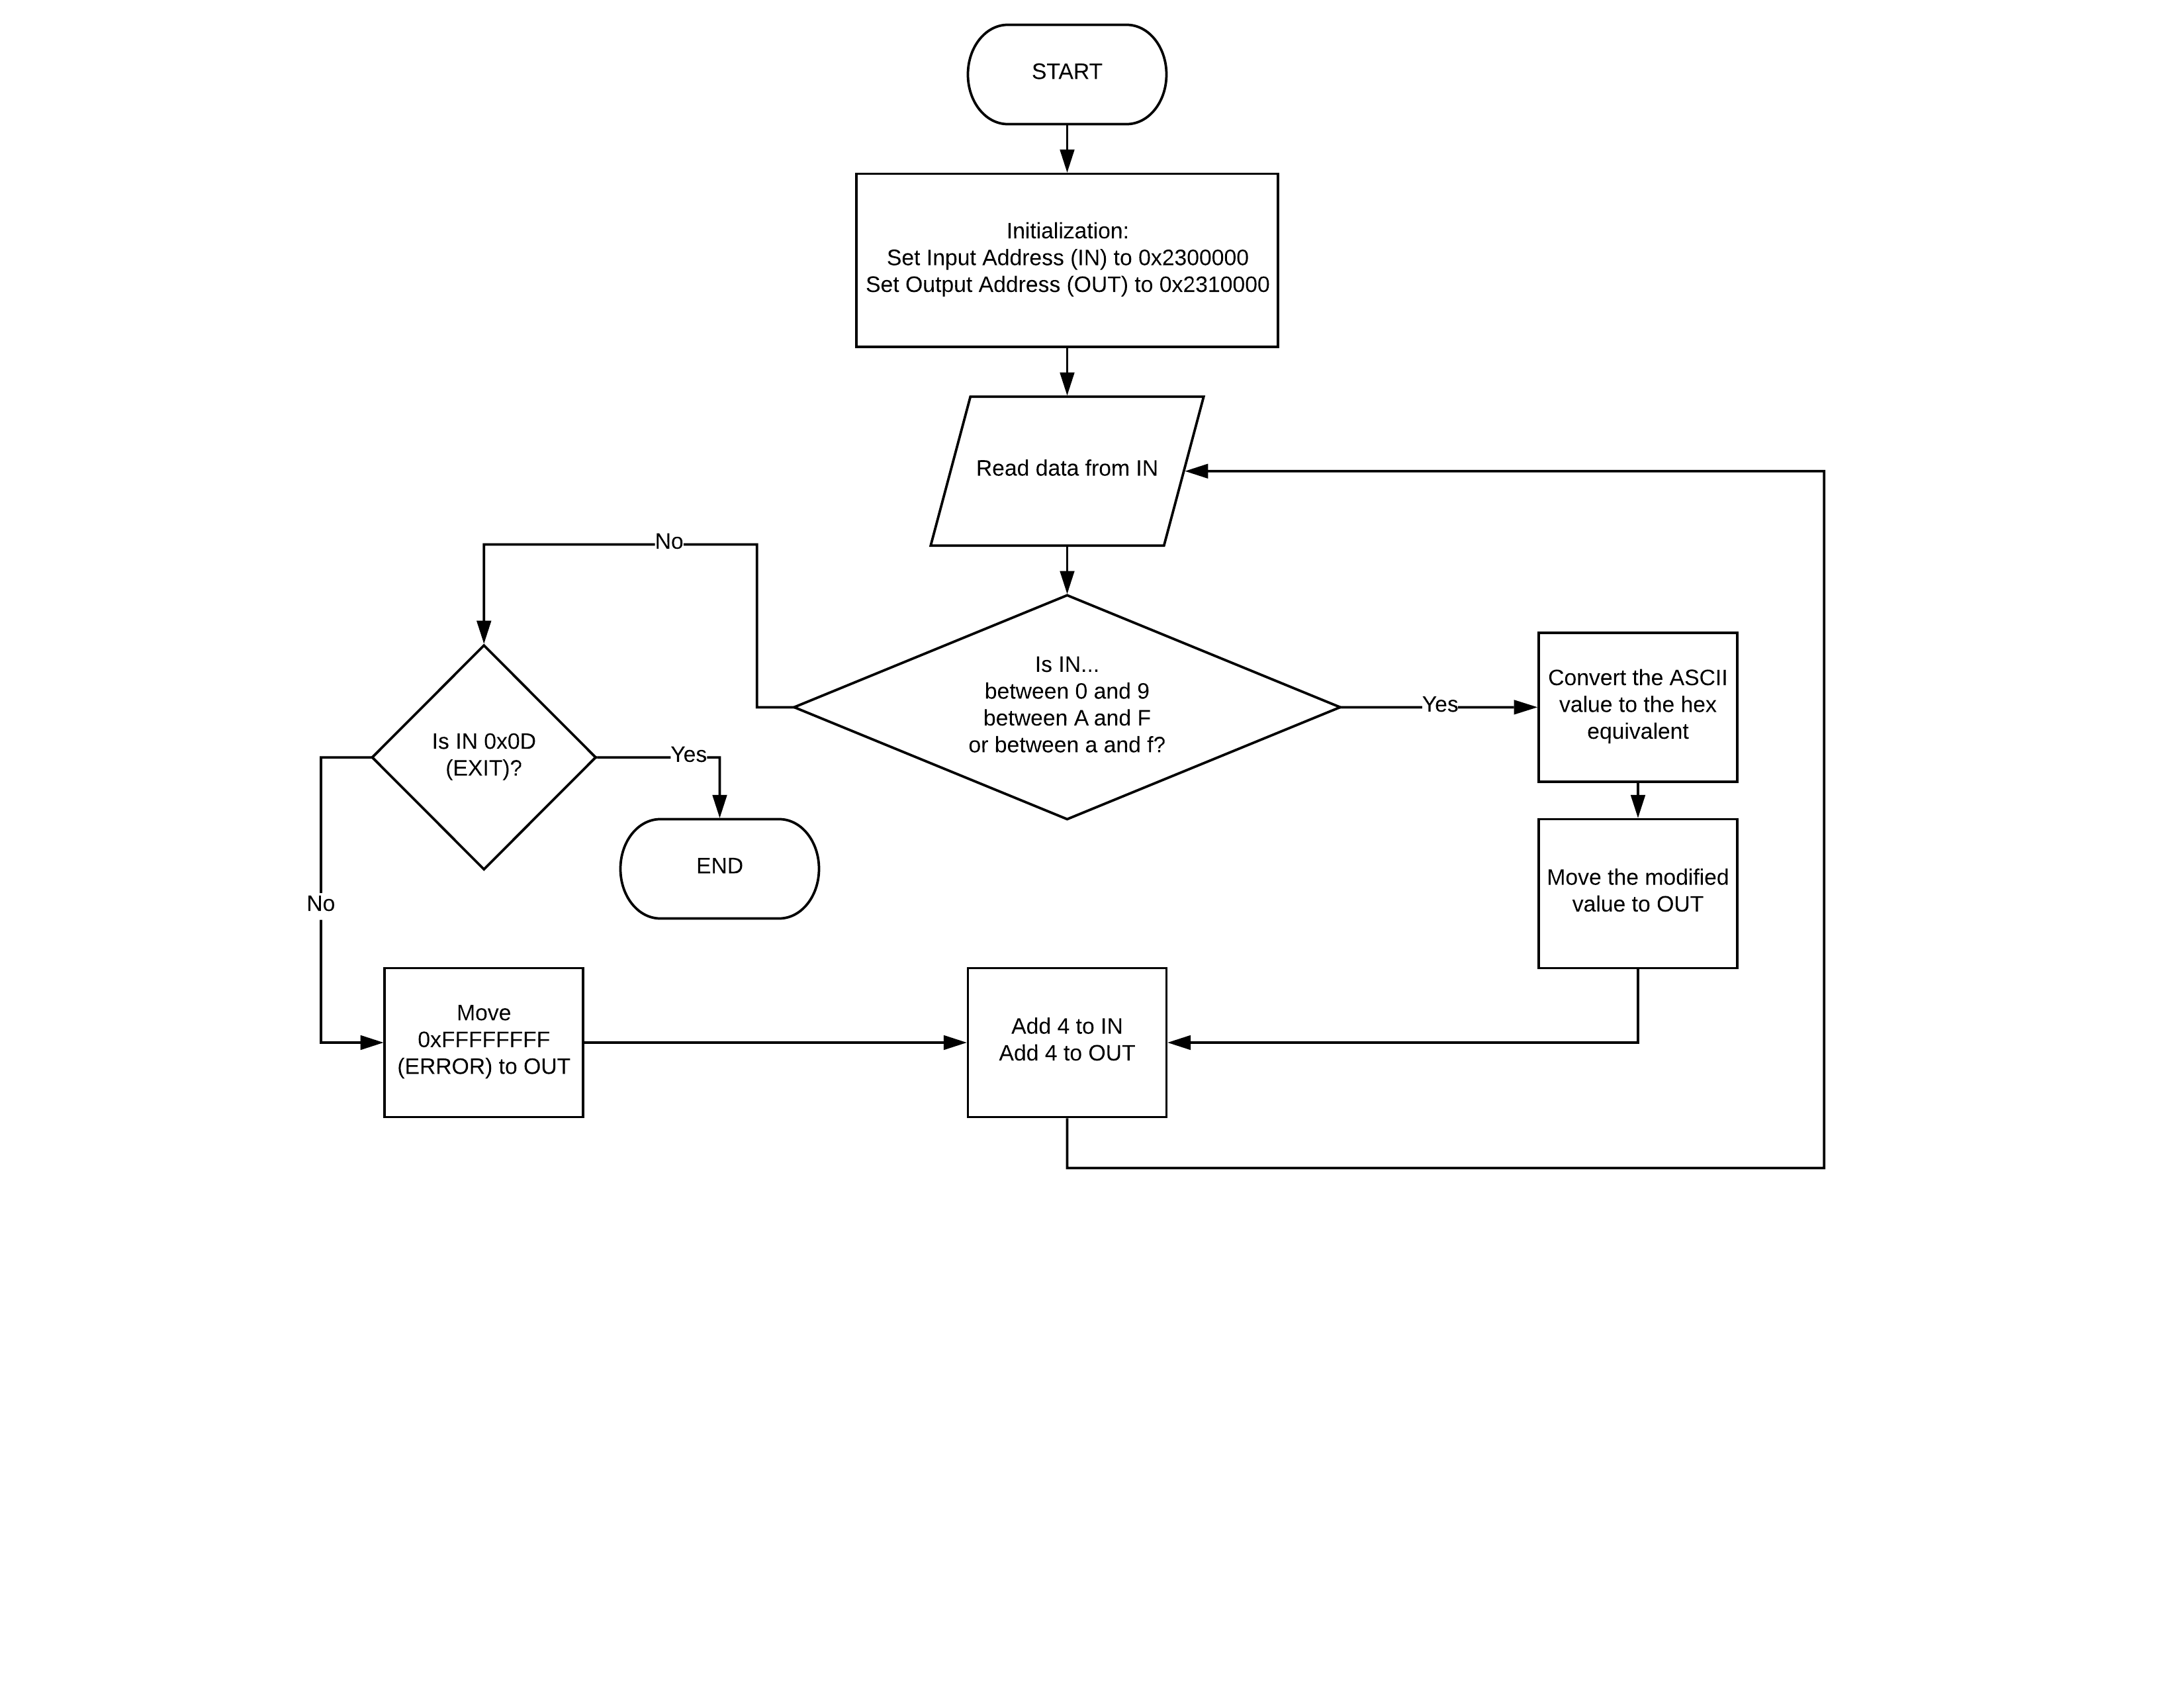
\includegraphics[width=0.4\textwidth]{partaflowchart.png}
      \caption{Flowchart for Part A}
    \end{figure}
\newpage
  \subsection{Part B Assembler Code}
    \lstinputlisting{partb.s}
\newpage
  \subsection{Part B Flowchart Diagram}
    \begin{figure}[h!]
      \centering
      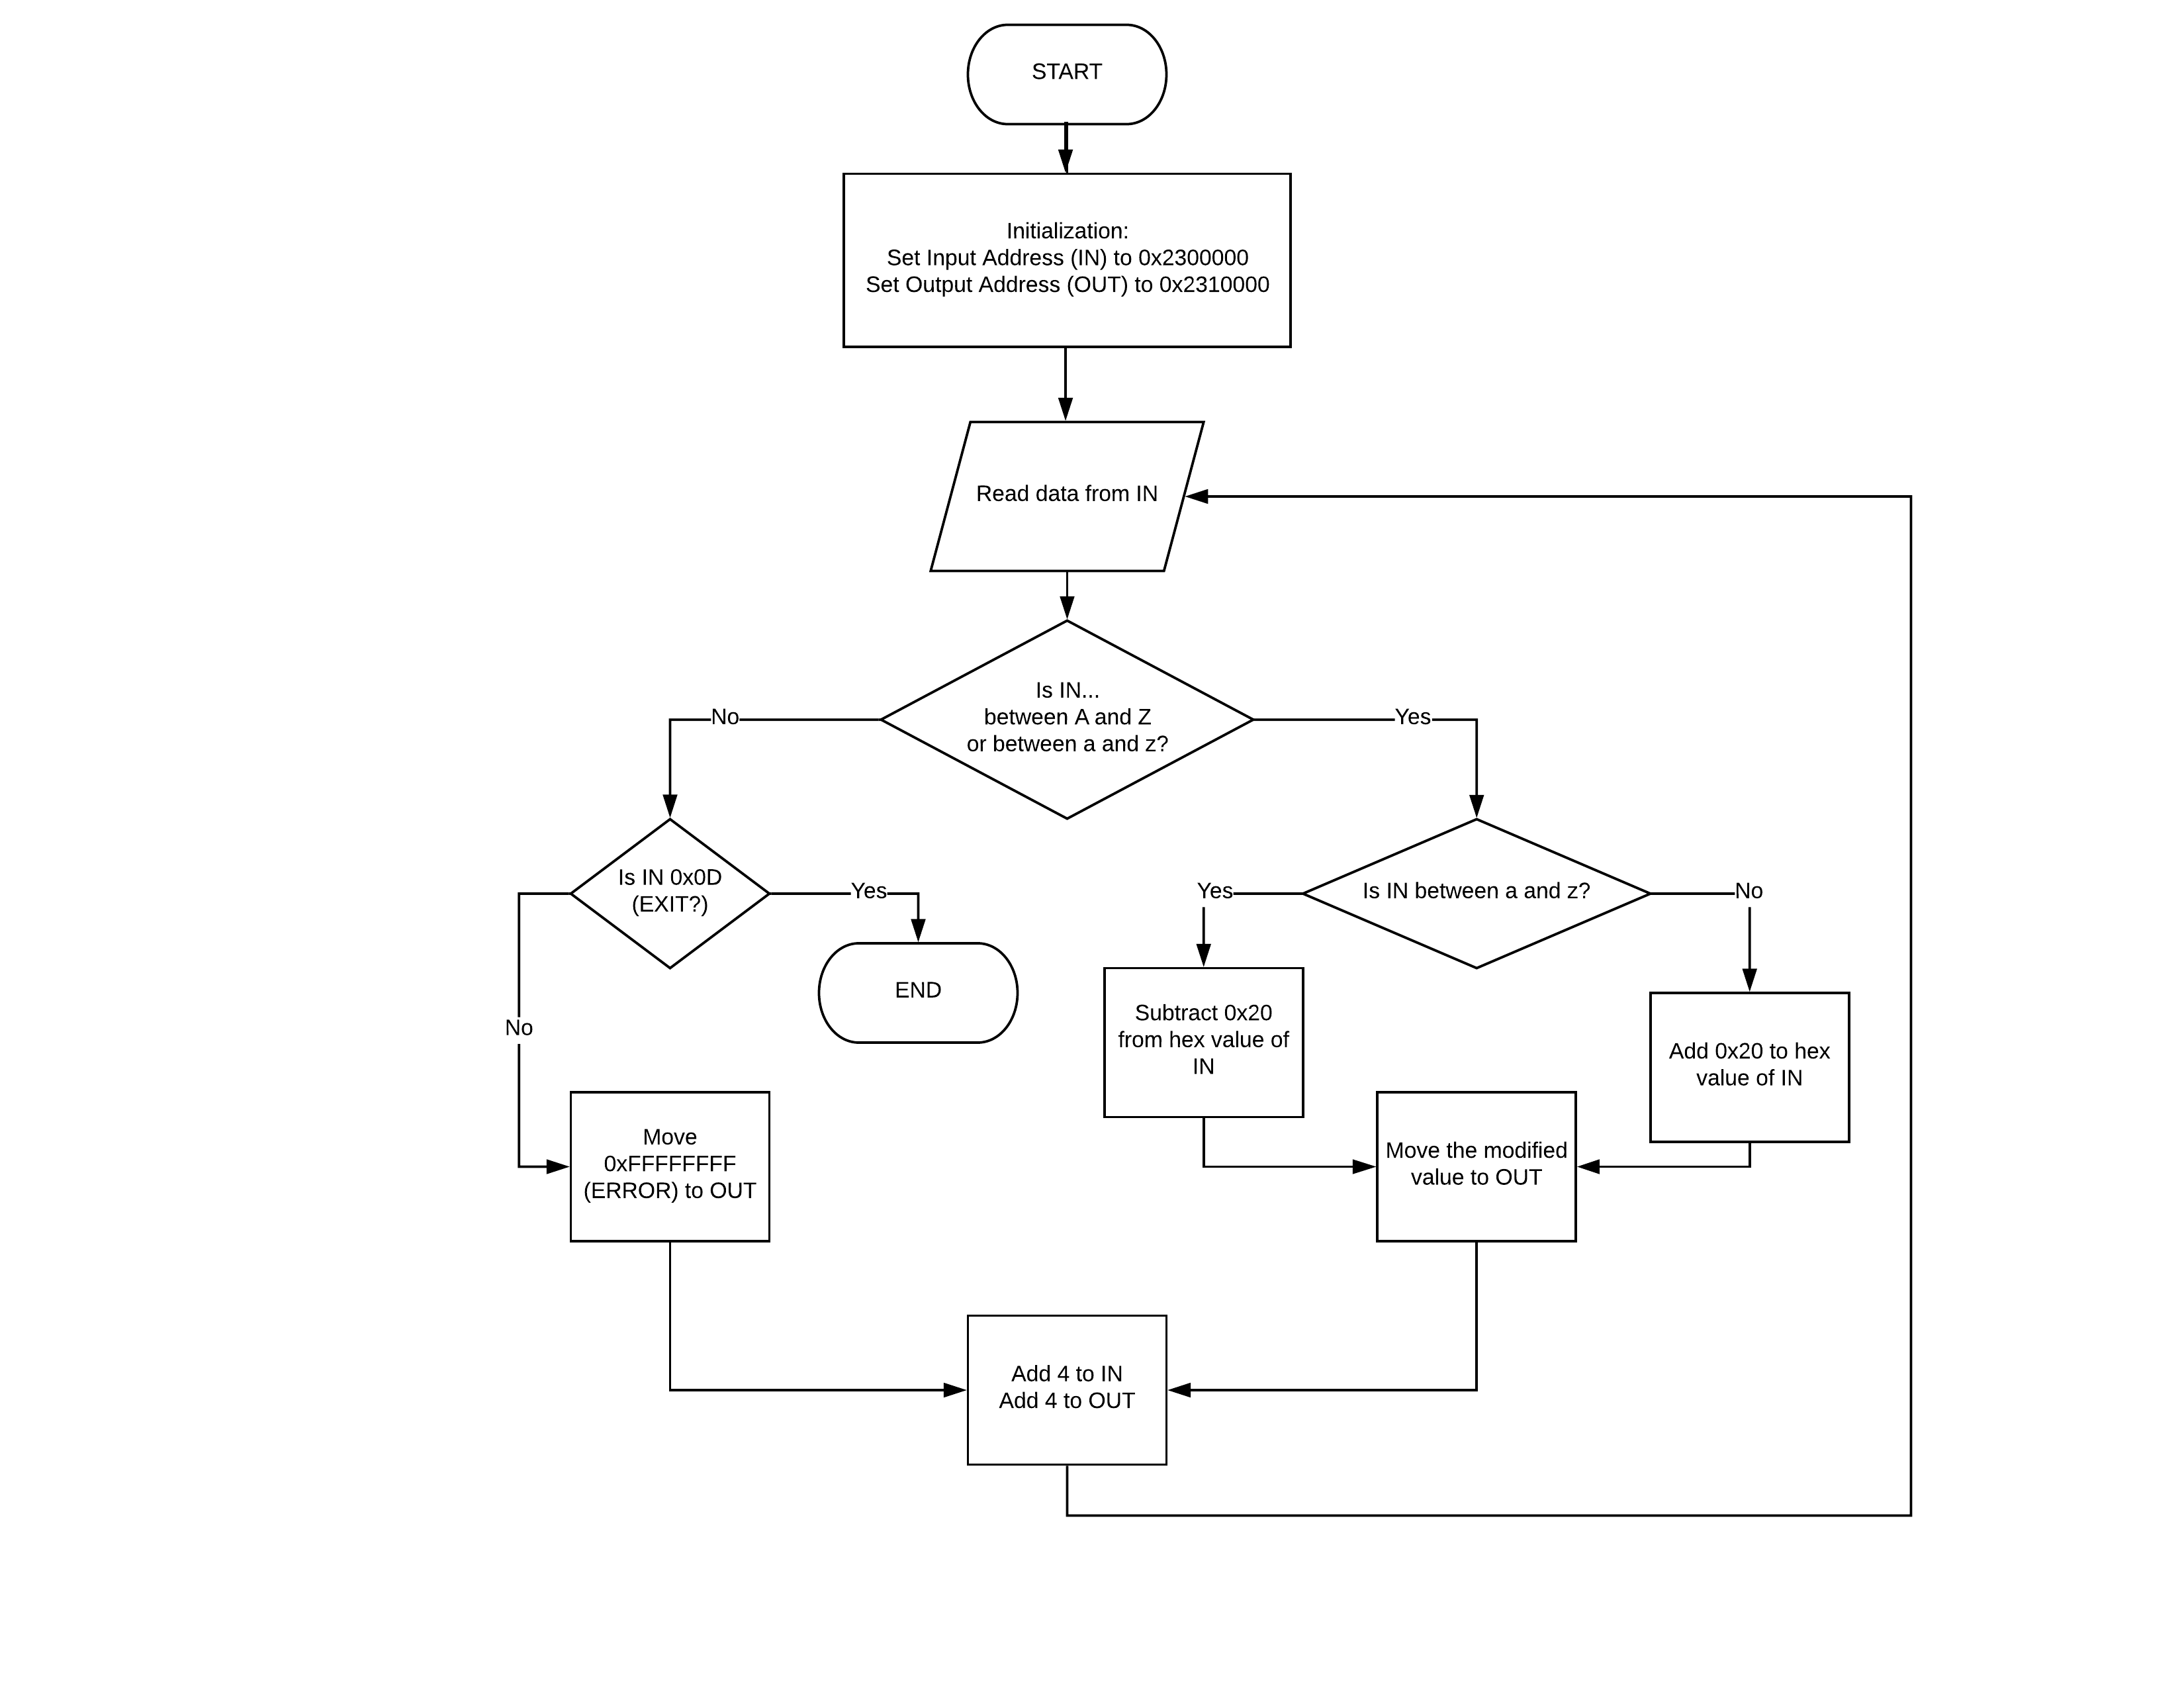
\includegraphics[width=0.4\textwidth]{partbflowchart.png}
      \caption{Flowchart for Part B}
    \end{figure}
\newpage
% \@
% % \pagenumbering{gobble}
% % \addcontentsline{toc}{section}{Marking Sheet}
% % \section{Marking Sheet}
% % \clearpage
% \addtocounter{section}{1}
% % \addcontentsline{toc}{section}{Marking Sheet}
% \addcontentsline{toc}{section}{\protect\numberline{\thesection} Marking Sheet}

\section{Marking Sheet}
\end{document}
